\chapter{Etat de l'art}

\section{Différents type de données}
Pour réaliser notre projet : animer un modèle de main en se basant sur les mouvements de la main de l'utilisateur, nous avons à disposition une 
Kinect 2 et un LeapMotion. Pour commencer notre état de l'art, nous allons voir quelles données peuvent être récupérées par ces outils et 
quels autres moyens auraient pu être utilisés pour réaliser ce projet.\\

Une liste non exhaustive des périphériques et des données utile qu'ils fournissent : 
\begin{itemize}
\item Kinect et Kinect 2 de Microsoft, fournissent en données brutes une image RGB ainsi qu'une image de profondeur. 
En utilisant le SDK fournis, on dispose en plus nombreux outils parmi lesquels une détection du squelette et pour Kinect 2 
une abstraction de la main avec 3 points détectés : le centre du poignet, le sommet de pouce et le sommet du majeur. 
\item LeapMotion et LeapMotion 2, fournissent en données brutes une image de profondeur plus détaillée mais sur une zone 
plus restreinte. Avec le SDK, on a accès à 
%% TODO se renseigner sur le SDK et la technologie LeapMotion
\item RealSense 
\end{itemize}
\ \\
Les données en RGB peuvent être utiliser avec des accessoires pour utilisées pour simplifier la détection des points de la main. \cite{wang2009real} 
Elles peuvent également être associées avec des données de profondeur pour améliorer la détection et gérer les cas de superposition \cite{van2011combining}

\section{Modélisation de la main}
%input
Pour mieux visualiser les actions réalisées par la main de l'utilisateur, il est nécessaire d'avoir
un modèle de la main qui soit réaliste et précis par rapport à la réalité. Pour cela, nous avons besoin d'un
mesh d'une main modèle que nous allons ensuite adapté à la main de l'utilisateur.\\

%icp
La méthode utilisé par \cite{export:217428} permet en utilisant l'algorithme
ICP\footnote{Iterated Closest Point} \cite{121791} de modifier le mesh de la main afin
que les points de celui-ci aient une distance moins importante avec le nuage de point fourni pas la 
caméra. Pour cela, l'algorithme ICP recherche les transformations, rotation et translation, qui permettent 
à partir d'un mesh M d'obtenir un mesh P. Dans notre cas, le mesh M représente le modèle de main donné en entré
et le mesh P représente la main de l'utilisateur.\\ 

%squelette TODO trop dur
La méthode de \cite{export:217428} permet également d'adapter le squelette du modèle de la 
main, ce qui permet d'obtenir une précision plus importante lors de l'utilisation de l'application.
Cette méthode se repose sur le calcul de la fonction énergie.

\section{Détection de la main}
\subsection{Construction d'une ROI}
Pour réaliser la détection de la main, il faut dans un premier temps déterminer une ROI\footnote{Region Of Interest}
autour ce celle-ci. Cette première étape a été expliqué dans \cite{export:238453}, où les auteurs utilise un classifieur
qui se repose sur la méthode développé dans \cite{export:145347}. Ce classifieur permet d'effectuer de la reconnaissance
des parties du corps et permet également de détecter les articulations.

\begin{figure}[!h]
 \begin{center}
  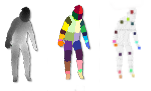
\includegraphics[width=5cm]{images/bodyrecognition.png}
  \caption{Résultat de la détection des parties du corps et des articulations grâce à la méthode de \cite{export:145347}}
  \label{fig:bodyrecognition}
 \end{center}
\end{figure}

On voit sur la Fig. \ref{fig:bodyrecognition} que l'articulation de la main est détecté, il est alors possible de construire
une ROI autour de ce point. Cette méthode est a été implémenté dans la caméra Kinect.

\subsection{Détection des mouvements de la main}
La méthode utilisé dans \cite{export:238453} ne nécessite aucune donnée provenant d'image antérieur. L'ensemble
des calculs sont réalisés sur une image à partir d'une base de connaissance contenant différente posture de la
main. Etant donnée qu'il est impossible de stocker toutes les postures de la main, la méthode de \cite{export:238453}
calcule une fonction energy permettant de déterminer quel est la posture la plus représentative de celle de la main
de l'utilisateur.

\section{Evaluation des solutions envisagées}
